\documentclass[../main.tex]{subfiles}

\begin{document}
\begin{problema}
	Consider a platform that is rotating about the \(z\)-axis with
	constant angular velocity \(\omega = \omega \uvec{k}\) in the
	inertial reference frame \(\mathcal{O}\). Let \(\mathcal{O}^{\prime}\)
	denote a reference frame that is rotating with the platform.
	An object of mass \(m\) is connected to a string that is pulled
	radially inward along the surface of the platform a t a
	constant speed \(v\) in \( \mathcal{O}^{\prime}\). At the instant
	shown in \zcref{fig:problem04}, the object is at a distance \(r = r^{\prime}\)
	from the center of the platform. What is the velocity of
	the object \(v\) in the reference frame \(\mathcal{O}\)?

	\begin{figure}[htb]
		\centering
		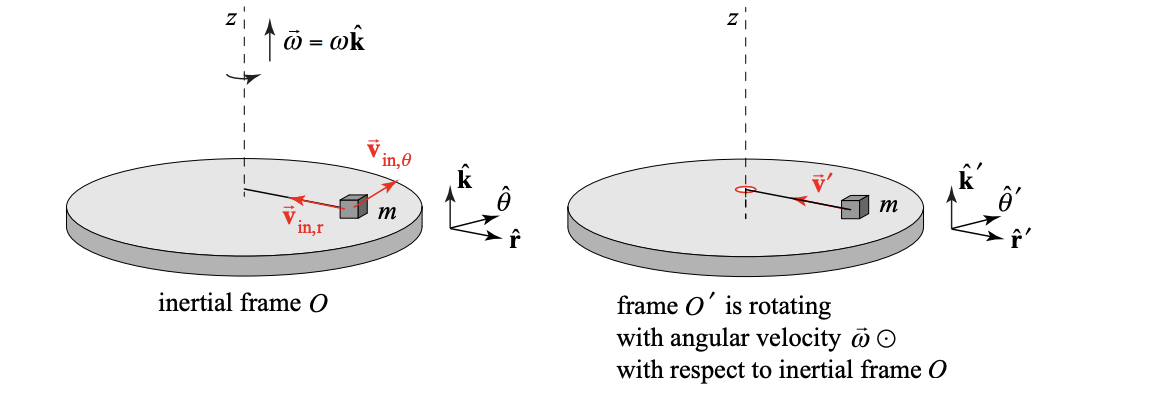
\includegraphics[width=0.45\textwidth]{figs/problema04.png}
		\caption{Reference systems \(\mathcal{O}\) and \(\mathcal{O}^{\prime}\).}
		\label{fig:problem04}
	\end{figure}
\end{problema}
\end{document}
